\begin{figure}[!htbp]
\begin{minipage}[b]{.5\linewidth}
\centering
\resizebox{\textwidth}{!}{
   % This file was created by tikzplotlib v0.9.8.
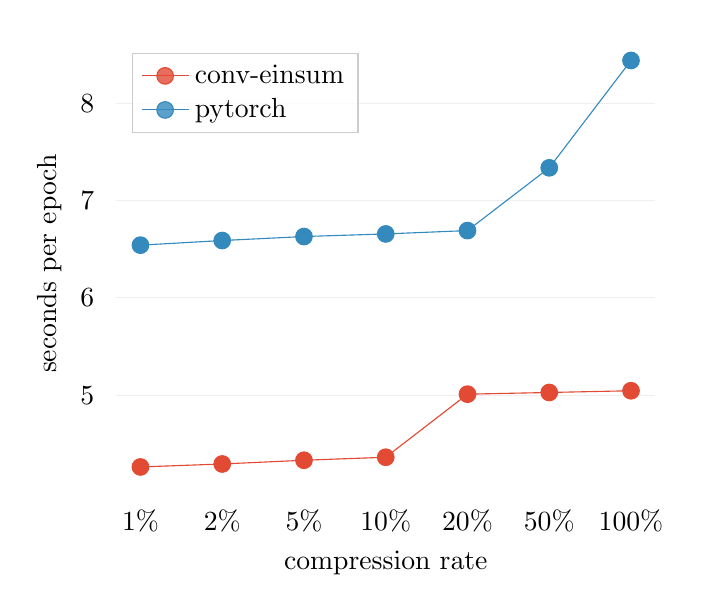
\begin{tikzpicture}

\definecolor{color0}{rgb}{0.886274509803922,0.290196078431373,0.2}
\definecolor{color1}{rgb}{0.203921568627451,0.541176470588235,0.741176470588235}

\begin{axis}[
axis line style={white},
legend cell align={left},
legend style={
  fill opacity=0.8,
  draw opacity=1,
  text opacity=1,
  at={(0.03,0.97)},
  anchor=north west,
  draw=white!80!black
},
tick align=outside,
x grid style={white},
xlabel={compression rate},
xmajorticks=true,
xtick style={draw=none},
xmin=0.7, xmax=7.3,
xtick style={color=white!33.3333333333333!black},
xtick={0,1,2,3,4,5,6,7,8},
xticklabels={,1\%,2\%,5\%,10\%,20\%,50\%,100\%,},
y grid style={white!93.3333333333333!black},
ylabel={seconds per epoch},
ymajorgrids,
ymajorticks=true,
ytick style={draw=none},
ymin=4.0504757670294, ymax=8.65358857814396,
ytick style={color=white!33.3333333333333!black}
]
\path [fill=color0, fill opacity=0.2, very thin]
(axis cs:1,4.2690774709811)
--(axis cs:1,4.25970816753461)
--(axis cs:2,4.29285513764861)
--(axis cs:3,4.3312428512991)
--(axis cs:4,4.35870023922928)
--(axis cs:5,5.00634535320453)
--(axis cs:6,5.02738922660089)
--(axis cs:7,5.04549989705764)
--(axis cs:7,5.04821726999854)
--(axis cs:7,5.04821726999854)
--(axis cs:6,5.03085050296498)
--(axis cs:5,5.01655082428636)
--(axis cs:4,4.36931002758693)
--(axis cs:3,4.33578040572975)
--(axis cs:2,4.29711997813592)
--(axis cs:1,4.2690774709811)
--cycle;

\path [fill=color1, fill opacity=0.2, very thin]
(axis cs:1,6.5432563125808)
--(axis cs:1,6.54022242597505)
--(axis cs:2,6.58484880369096)
--(axis cs:3,6.62930560515728)
--(axis cs:4,6.65497483141372)
--(axis cs:5,6.68958406774542)
--(axis cs:6,7.33483066502077)
--(axis cs:7,8.43179643541149)
--(axis cs:7,8.44435617763875)
--(axis cs:7,8.44435617763875)
--(axis cs:6,7.33662622615381)
--(axis cs:5,6.69343568179097)
--(axis cs:4,6.65906086290792)
--(axis cs:3,6.6316352477383)
--(axis cs:2,6.59456363074972)
--(axis cs:1,6.5432563125808)
--cycle;

\addplot [color0, mark=*, mark size=3, mark options={solid}]
table {%
1 4.26440201503572
2 4.29491886427219
3 4.33342431321434
4 4.36409679450395
5 5.01176841479325
6 5.02916789812413
7 5.04686331290392
};
\addlegendentry{conv-einsum}
\addplot [color1, mark=*, mark size=3, mark options={solid}]
table {%
1 6.54178683473819
2 6.5893361431478
3 6.63039308645571
4 6.65699675146461
5 6.69144116037216
6 7.3357529608339
7 8.43806635143422
};
\addlegendentry{pytorch}
\end{axis}

\end{tikzpicture}

    }
\subcaption{CP Train}\label{fig:imagecls-cp-vs-pytorch-train}
\end{minipage}%
\hfill
\begin{minipage}[b]{.5\linewidth}
\centering
\resizebox{\textwidth}{!}{
    % This file was created by tikzplotlib v0.9.8.
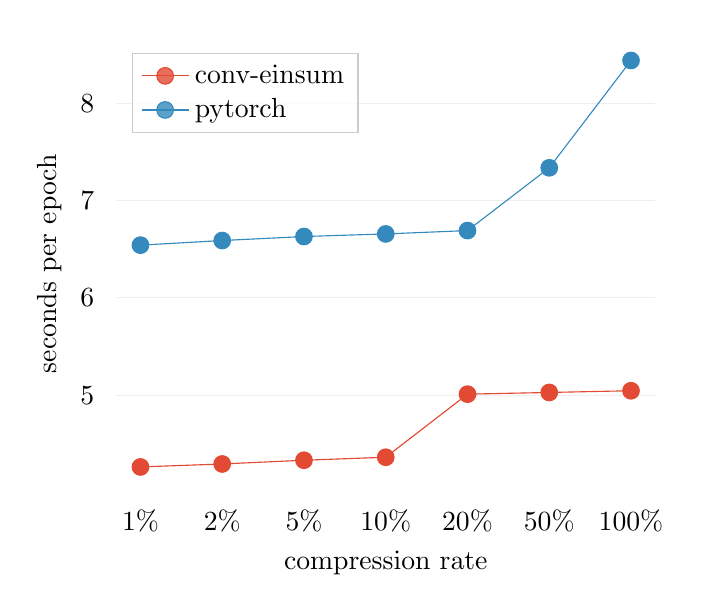
\begin{tikzpicture}

\definecolor{color0}{rgb}{0.886274509803922,0.290196078431373,0.2}
\definecolor{color1}{rgb}{0.203921568627451,0.541176470588235,0.741176470588235}

\begin{axis}[
axis line style={white},
legend cell align={left},
legend style={
  fill opacity=0.8,
  draw opacity=1,
  text opacity=1,
  at={(0.03,0.97)},
  anchor=north west,
  draw=white!80!black
},
tick align=outside,
x grid style={white},
xlabel={compression rate},
xmajorticks=true,
xtick style={draw=none},
xmin=0.7, xmax=7.3,
xtick style={color=white!33.3333333333333!black},
xtick={0,1,2,3,4,5,6,7,8},
xticklabels={,1\%,2\%,5\%,10\%,20\%,50\%,100\%,},
y grid style={white!93.3333333333333!black},
ylabel={seconds per epoch},
ymajorgrids,
ymajorticks=true,
ytick style={draw=none},
ymin=4.05004441746139, ymax=8.65361560922929,
ytick style={color=white!33.3333333333333!black}
]
\path [fill=color0, fill opacity=0.2, very thin]
(axis cs:1,4.26919628104229)
--(axis cs:1,4.25929765345084)
--(axis cs:2,4.29276170704354)
--(axis cs:3,4.33114307693408)
--(axis cs:4,4.35883259883012)
--(axis cs:5,5.00652041823997)
--(axis cs:6,5.02760501921923)
--(axis cs:7,5.04550376414628)
--(axis cs:7,5.04839590362911)
--(axis cs:7,5.04839590362911)
--(axis cs:6,5.030967426714)
--(axis cs:5,5.01672765765548)
--(axis cs:4,4.36918221123034)
--(axis cs:3,4.33585936784547)
--(axis cs:2,4.29709082160542)
--(axis cs:1,4.26919628104229)
--cycle;

\path [fill=color1, fill opacity=0.2, very thin]
(axis cs:1,6.54315019234397)
--(axis cs:1,6.54036059319545)
--(axis cs:2,6.58477810534335)
--(axis cs:3,6.62930560515727)
--(axis cs:4,6.65497483141372)
--(axis cs:5,6.68973749279177)
--(axis cs:6,7.33470682756735)
--(axis cs:7,8.43117219428478)
--(axis cs:7,8.44436237323984)
--(axis cs:7,8.44436237323984)
--(axis cs:6,7.33664540912606)
--(axis cs:5,6.6932080261672)
--(axis cs:4,6.65907224231569)
--(axis cs:3,6.63132416377561)
--(axis cs:2,6.59530051772351)
--(axis cs:1,6.54315019234397)
--cycle;

\addplot [color0, mark=*, mark size=3, mark options={solid}]
table {%
1 4.26432893183369
2 4.2948522928311
3 4.33339123674121
4 4.36398843227655
5 5.01190894389394
6 5.02919161379351
7 5.04687747252056
};
\addlegendentry{conv-einsum}
\addplot [color1, mark=*, mark size=3, mark options={solid}]
table {%
1 6.54179353891074
2 6.58928042365596
3 6.63037029318219
4 6.65701421927132
5 6.69144051071459
6 7.33575286680573
7 8.43803039052754
};
\addlegendentry{pytorch}
\end{axis}

\end{tikzpicture}

    }
\subcaption{CP Test}\label{fig:imagecls-cp-vs-pytorch-test}
\end{minipage}
\caption{Run-time comparison between \texttt{conv\_einsum} and \texttt{Pytorch} implementation of CP-TNN for image classification machine learning task implemented on CIFAR-10 dataset. We denote error bars using shaded areas and they are generated using 10 random runs. }\label{fig:imagecls-cp-vs-pytorch}
\end{figure}